
\documentclass[tikz,border=10pt]{standalone}
\begin{document}
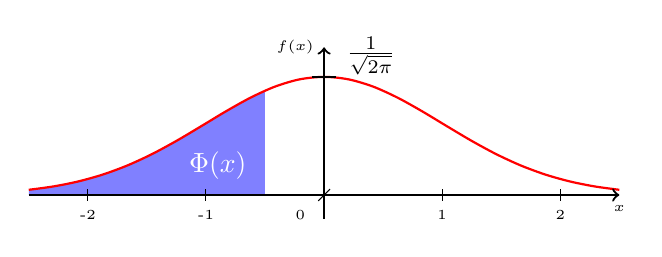
\begin{tikzpicture}[scale=1.5]
	% Schraffur
	\fill[domain=-2.5:-0.5, color=red, thick, smooth, fill=blue!50]
    	plot (\x, {exp((\x * \x) / -2)}) -- (-0.5,0) --(-2.5,0);
    % Beschriftung
    \draw (-0.9,0.25) node[color=white] {$\Phi(x)$};
    % Plot    
	\draw[domain=-2.5:2.5, smooth, thick, color=red]
    plot (\x,{exp((\x * \x)/ -2)});
    % Achsen
    \draw[->, thick] (-2.5,0) -- (2.5,0) node[below] {\tiny{$x$}};
    \draw[->, thick] (0,-0.2) -- (0,1.25) node[left] {\tiny{$f(x)$}};
    % Achsenskalierung
    \draw[thick] (-0.1,1) -- (0.1,1) node[right, yshift=0.75em] {$\frac{1}{\sqrt{2\pi}}$};
    \foreach \x in {-2,-1,1,2}
    	\draw[xshift=\x cm] (0.0,0.05) -- (0.0,-0.05) node[below]{\tiny{\x}};
    \draw (0.05,0.05) -- (-0.05,-0.05) node[below, xshift=-1.5ex] {\tiny{0}};
\end{tikzpicture}
\end{document}